%-----------------------------------------------------------------------------------------------------------------------------------------------%
%  The MIT License (MIT)
%
%  Copyright (c) 2019 Jan Küster
%
%  Permission is hereby granted, free of charge, to any person obtaining a copy
%  of this software and associated documentation files (the "Software"), to deal
%  in the Software without restriction, including without limitation the rights
%  to use, copy, modify, merge, publish, distribute, sublicense, and/or sell
%  copies of the Software, and to permit persons to whom the Software is
%  furnished to do so, subject to the following conditions:
%
%  THE SOFTWARE IS PROVIDED "AS IS", WITHOUT WARRANTY OF ANY KIND, EXPRESS OR
%  IMPLIED, INCLUDING BUT NOT LIMITED TO THE WARRANTIES OF MERCHANTABILITY,
%  FITNESS FOR A PARTICULAR PURPOSE AND NONINFRINGEMENT. IN NO EVENT SHALL THE
%  AUTHORS OR COPYRIGHT HOLDERS BE LIABLE FOR ANY CLAIM, DAMAGES OR OTHER
%  LIABILITY, WHETHER IN AN ACTION OF CONTRACT, TORT OR OTHERWISE, ARISING FROM,
%  OUT OF OR IN CONNECTION WITH THE SOFTWARE OR THE USE OR OTHER DEALINGS IN
%  THE SOFTWARE.
%
%
%-----------------------------------------------------------------------------------------------------------------------------------------------%


%============================================================================%
%
%  DOCUMENT DEFINITION
%
%============================================================================%

\documentclass[10pt,A4,english]{article}


%----------------------------------------------------------------------------------------
%  ENCODING
%----------------------------------------------------------------------------------------

% we use utf8 since we want to build from any machine
\usepackage[utf8]{inputenc}
\usepackage[USenglish]{isodate}
\usepackage{fancyhdr}
\usepackage[numbers]{natbib}

%----------------------------------------------------------------------------------------
%  LOGIC
%----------------------------------------------------------------------------------------

% provides \isempty test
\usepackage{xstring, xifthen}
\usepackage{enumitem}
\usepackage[francais]{babel}
\usepackage{blindtext}
\usepackage{pdfpages}
\usepackage{changepage}
%----------------------------------------------------------------------------------------
%  FONT BASICS
%----------------------------------------------------------------------------------------

% some tex-live fonts - choose your own

%\usepackage[defaultsans]{droidsans}
%\usepackage[default]{comfortaa}
%\usepackage{cmbright}
\usepackage[default]{raleway}
%\usepackage{fetamont}
%\usepackage[default]{gillius}
%\usepackage[light,math]{iwona}
%\usepackage[thin]{roboto}

% set font default
\renewcommand*\familydefault{\sfdefault}
\usepackage[T1]{fontenc}

% more font size definitions
\usepackage{moresize}

%----------------------------------------------------------------------------------------
%  FONT AWESOME ICONS
%----------------------------------------------------------------------------------------

% include the fontawesome icon set
\usepackage{fontawesome}

% use to vertically center content
% credits to: http://tex.stackexchange.com/questions/7219/how-to-vertically-center-two-images-next-to-each-other
\newcommand{\vcenteredinclude}[1]{\begingroup
  \setbox0=\hbox{\includegraphics{#1}}%
\parbox{\wd0}{\box0}\endgroup}
\newcommand{\tab}[1]{\hspace{.2\textwidth}\rlap{#1}}
% use to vertically center content
% credits to: http://tex.stackexchange.com/questions/7219/how-to-vertically-center-two-images-next-to-each-other
\newcommand*{\vcenteredhbox}[1]{\begingroup
\setbox0=\hbox{#1}\parbox{\wd0}{\box0}\endgroup}

% icon shortcut
\newcommand{\icon}[3] {
  \makebox(#2, #2){\textcolor{maincol}{\csname fa#1\endcsname}}
}


% icon with text shortcut
\newcommand{\icontext}[4]{
  \vcenteredhbox{\icon{#1}{#2}{#3}}  \hspace{2pt}  \parbox{0.9\mpwidth}{\textcolor{#4}{#3}}
}

% icon with website url
\newcommand{\iconhref}[5]{
  \vcenteredhbox{\icon{#1}{#2}{#5}}  \hspace{2pt} \href{#4}{\textcolor{#5}{#3}}
}

% icon with email link
\newcommand{\iconemail}[5]{
  \vcenteredhbox{\icon{#1}{#2}{#5}}  \hspace{2pt} \href{mailto:#4}{\textcolor{#5}{#3}}
}

%----------------------------------------------------------------------------------------
%  PAGE LAYOUT  DEFINITIONS
%----------------------------------------------------------------------------------------

% page outer frames (debug-only)
% \usepackage{showframe}

% we use paracol to display breakable two columns
\usepackage{paracol}
\usepackage{tikzpagenodes}
\usetikzlibrary{calc}
\usepackage{lmodern}
\usepackage{multicol}
\usepackage{lipsum}
\usepackage{atbegshi}
% define page styles using geometry
\usepackage[a4paper]{geometry}

% remove all possible margins
\geometry{top=1cm, bottom=1cm, left=1cm, right=1cm}

\usepackage{fancyhdr}
\pagestyle{empty}

% space between header and content
% \setlength{\headheight}{0pt}

% indentation is zero
\setlength{\parindent}{0mm}

%----------------------------------------------------------------------------------------
%  TABLE /ARRAY DEFINITIONS
%----------------------------------------------------------------------------------------

% extended aligning of tabular cells
\usepackage{array}

% custom column right-align with fixed width
% use like p{size} but via x{size}
\newcolumntype{x}[1]{%
>{\raggedleft\hspace{0pt}}p{#1}}%


%----------------------------------------------------------------------------------------
%  GRAPHICS DEFINITIONS
%----------------------------------------------------------------------------------------

%for header image
\usepackage{graphicx}

% use this for floating figures
% \usepackage{wrapfig}
% \usepackage{float}
% \floatstyle{boxed}
% \restylefloat{figure}

%for drawing graphics
\usepackage{tikz}
\usepackage{ragged2e}
\usetikzlibrary{shapes, backgrounds,mindmap, trees}

%----------------------------------------------------------------------------------------
%  Color DEFINITIONS
%----------------------------------------------------------------------------------------
\usepackage{transparent}
\usepackage{color}

% primary color
\definecolor{maincol}{RGB}{ 64,64,64}

% accent color, secondary
% \definecolor{accentcol}{RGB}{ 250, 150, 10 }

% dark color
\definecolor{darkcol}{RGB}{ 70, 70, 70 }

% light color
\definecolor{lightcol}{RGB}{245,245,245}

\definecolor{accentcol}{RGB}{59,77,97}



% Package for links, must be the last package used
\usepackage[hidelinks]{hyperref}

% returns minipage width minus two times \fboxsep
% to keep padding included in width calculations
% can also be used for other boxes / environments
\newcommand{\mpwidth}{\linewidth-\fboxsep-\fboxsep}



%============================================================================%
%
%  CV COMMANDS
%
%============================================================================%

%----------------------------------------------------------------------------------------
%   CV LIST
%----------------------------------------------------------------------------------------

% renders a standard latex list but abstracts away the environment definition (begin/end)
\newcommand{\cvlist}[1] {
  \begin{itemize}{#1}
  \end{itemize}
}

%----------------------------------------------------------------------------------------
%   CV TEXT
%----------------------------------------------------------------------------------------

% base class to wrap any text based stuff here. Renders like a paragraph.
% Allows complex commands to be passed, too.
% param 1: *any
\newcommand{\cvtext}[1] {
  \begin{tabular*}{1\mpwidth}{p{0.98\mpwidth}}
    \parbox{1\mpwidth}{#1}
  \end{tabular*}
}
\newcommand{\cvtextsmall}[1] {
  \begin{tabular*}{0.8\mpwidth}{p{0.8\mpwidth}}
    \parbox{0.8\mpwidth}{#1}
  \end{tabular*}
}
%----------------------------------------------------------------------------------------
%  CV SECTION
%----------------------------------------------------------------------------------------

% Renders a a CV section headline with a nice underline in main color.
% param 1: section title
\newlength{\barw}
\newcommand{\cvsection}[1] {
  \vspace{14pt}
  \settowidth{\barw}{\textbf{\LARGE #1}}
  \cvtext{
    \textbf{\LARGE{\textcolor{darkcol}{#1}}}\\[-4pt]
    \textcolor{accentcol}{ \rule{\barw}{1.5pt} } \\
  }
}

\newcommand{\cvsubsection}[1] {
  \vspace{14pt}
  \settowidth{\barw}{\textbf{\Large #1}}
  \cvtext{
    \textbf{\Large{\textcolor{darkcol}{#1}}}\\[-4pt]
    \textcolor{accentcol}{ \rule{\barw}{1.5pt} } \\
  }
}

\newcommand{\cvheadline}[1] {
  \vspace{16pt}
  \cvtext{
    \textbf{\Huge{\textcolor{accentcol}{#1}}}\\[-4pt]

  }
}

\newcommand{\cvsubheadline}[1] {
  \vspace{16pt}
  \cvtext{
    \textbf{\huge{\textcolor{darkcol}{#1}}}\\[-4pt]

  }
}
%----------------------------------------------------------------------------------------
%  META SKILL
%----------------------------------------------------------------------------------------

% Renders a progress-bar to indicate a certain skill in percent.
% param 1: name of the skill / tech / etc.
% param 2: level (for example in years)
% param 3: percent, values range from 0 to 1
\newcommand{\cvskill}[3] {
  \begin{tabular*}{1\mpwidth}{p{0.72\mpwidth}  r}
    \textcolor{black}{\textbf{#1}} & \textcolor{maincol}{#2}\\
  \end{tabular*}%

  \hspace{4pt}
  \begin{tikzpicture}[scale=1,rounded corners=2pt,very thin]
    \fill [lightcol] (0,0) rectangle (1\mpwidth, 0.15);
    \fill [accentcol] (0,0) rectangle (#3\mpwidth, 0.15);
  \end{tikzpicture}%
}


%----------------------------------------------------------------------------------------
%   CV EVENT
%----------------------------------------------------------------------------------------

% Renders a table and a paragraph (cvtext) wrapped in a parbox (to ensure minimum content
% is glued together when a pagebreak appears).
% Additional Information can be passed in text or list form (or other environments).
% the work you did
% param 1: time-frame i.e. Sep 14 - Jan 15 etc.
% param 2:   event name (job position etc.)
% param 3: Customer, Employer, Industry
% param 4: Short description
% param 5: work done (optional)
% param 6: technologies include (optional)
% param 7: achievements (optional)
\newcommand{\cvevent}[7] {

  % we wrap this part in a parbox, so title and description are not separated on a pagebreak
  % if you need more control on page breaks, remove the parbox
  \parbox{\mpwidth}{
    \begin{tabular*}{1\mpwidth}{p{0.66\mpwidth}  r}
      \textcolor{black}{\textbf{#2}} & \colorbox{accentcol}{\makebox[0.32\mpwidth]{\textcolor{white}{\textbf{#1}}}} \\
      \textcolor{maincol}{#3} & \\
    \end{tabular*}\\[8pt]

    \ifthenelse{\isempty{#4}}{}{
      \cvtext{#4}\\
    }
  }
  \vspace{14pt}
}


%----------------------------------------------------------------------------------------
%   CV META EVENT
%----------------------------------------------------------------------------------------

% Renders a CV event on the sidebar
% param 1: title
% param 2: subtitle (optional)
% param 3: customer, employer, etc,. (optional)
% param 4: info text (optional)
\newcommand{\cvmetaevent}[4] {
  \textcolor{black}{\cvtext{\textbf{#2}} }


  \cvtext{{\textcolor{maincol}{#3}}}

  \textcolor{maincol}{\cvtext{\textbf{#1}}}\\

  \cvtext{#4}\\[6pt]
}

%---------------------------------------------------------------------------------------
%  QR CODE
%----------------------------------------------------------------------------------------

% Renders a qrcode image (centered, relative to the parentwidth)
% param 1: percent width, from 0 to 1
\newcommand{\cvqrcode}[1] {
  \begin{center}
    \includegraphics[width={#1}\mpwidth]{qrcode}
  \end{center}
}


% HEADER AND FOOOTER
%====================================
\newcommand\Header[1]{%
  \begin{tikzpicture}[remember picture,overlay]
    \fill[accentcol]
    (current page.north west) -- (current page.north east) --
    ([yshift=50pt]current page.north east|-current page text area.north east) --
    ([yshift=50pt,xshift=-3cm]current page.north|-current page text area.north) --
    ([yshift=10pt,xshift=-5cm]current page.north|-current page text area.north) --
    ([yshift=10pt]current page.north west|-current page text area.north west) -- cycle;
    \node[font=\sffamily\bfseries\color{white},anchor=west,
    xshift=0.7cm,yshift=-0.32cm] at (current page.north west)
    {\fontsize{12}{12}\selectfont {#1}};
  \end{tikzpicture}%
}

\newcommand\Footer[1]{%
  \begin{tikzpicture}[remember picture,overlay]
    \fill[lightcol]
    (current page.south east) -- (current page.south west) --
    ([yshift=-80pt]current page.south east|-current page text area.south east) --
    ([yshift=-80pt,xshift=-6cm]current page.south|-current page text area.south) --
    ([xshift=-2.5cm,yshift=-10pt]current page.south|-current page text area.south) --
    ([yshift=-10pt]current page.south east|-current page text area.south east) -- cycle;
    \node[yshift=0.32cm,xshift=9cm] at (current page.south) {\fontsize{10}{10}\selectfont \textbf{\thepage}};
  \end{tikzpicture}%
}


%=====================================
%============================================================================%
%
%
%
%  DOCUMENT CONTENT
%
%
%
%============================================================================%
\begin{document}

\columnratio{0.31}
\setlength{\columnsep}{2.2em}
\setlength{\columnseprule}{4pt}
\colseprulecolor{white}


\AtBeginShipoutFirst{\Header{Curriculum Vitæ}\Footer{1}}
\AtBeginShipout{\AtBeginShipoutAddToBox{\Header{Curriculum Vitæ}\Footer{2}}}

\newpage

\colseprulecolor{lightcol}
\columnratio{0.31}
\setlength{\columnsep}{2.2em}
\setlength{\columnseprule}{4pt}
\begin{paracol}{2}


  \begin{leftcolumn}
    %---------------------------------------------------------------------------------------
    %  META IMAGE
    %----------------------------------------------------------------------------------------
    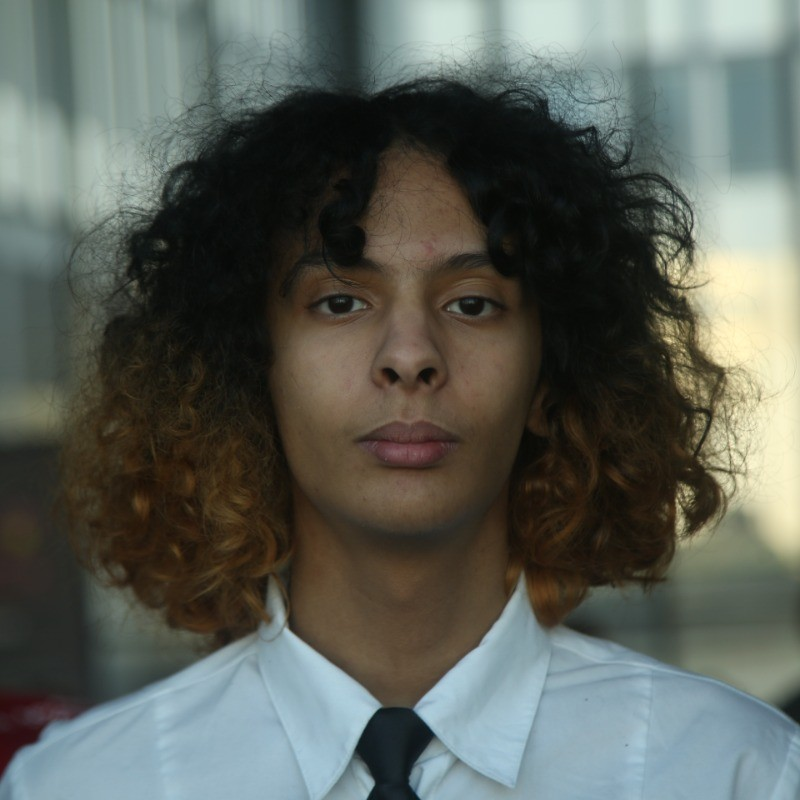
\includegraphics[width=\linewidth]{../assets/profile.jpg}  %trimming relative to image size

    \vspace{5pt}

    %---------------------------------------------------------------------------------------
    %  META SKILLS
    %----------------------------------------------------------------------------------------
    \fcolorbox{white}{white}{
      \begin{minipage}[c][1.5cm][c]{1\mpwidth}
        \LARGE{\textbf{\textcolor{maincol}{Boudrouss Réda}}} \\[2pt]
        \normalsize{ \textcolor{black} {Développeur Web \& Logiciel} }
    \end{minipage}} \\
    \icontext{CaretRight}{12}{Né le 12/07/2002 à Meknes, Maroc}{black}\\[6pt]
    \icontext{CaretRight}{12}{\textbf{Langues} : Français, Anglais (C1), Arabe}{black}\\[6pt]

    %---------------------------------------------------------------------------------------
    %  EDUCATION
    %----------------------------------------------------------------------------------------
    \cvsection{Études}

    \cvmetaevent
    {09/2024 - 07/2026}
    {• Master Science et Technologie du Logiciel}
    {Sorbonne Université - Jussieu}
    {\textit{Programmation Concurente Répartie Réactive • Composants • Fonctionnel Avancé}}

    \cvmetaevent
    {09/2020 - 07/2024}
    {• Licence d'informatique}
    {Sorbonne Université - Jussieu}
    {\textit{Base de donnée • Algorithmie • Technologie Web • IA \& jeu • Réseaux • Statistiques • OS}}

    \cvmetaevent
    {2020}
    {• Baccaulauréat Scientifique}
    {Lycée Paul Valéry - Meknes, Maroc}
    {}


    %---------------------------------------------------------------------------------------
    % Contact
    %----------------------------------------------------------------------------------------
    \cvsection{Contact}

    \icontext{MapMarker}{16}{Paris 13}{black}\\[6pt]
    \icontext{MobilePhone}{16}{+33 7 55 78 85 16}{black}\\[6pt]
    \iconemail{Envelope}{16}{contact@rboud.com}{contact@rboud.com}{black}\\[6pt]
    \iconhref{Github}{16}{github.com/rboudrouss}{https://www.github.com/rboudrouss}{black}\\[6pt]
    \iconhref{Home}{16}{rboud.com}{https://rboud.com}{black}\\[6pt]

  \end{leftcolumn}

  \begin{rightcolumn}

    %---------------------------------------------------------------------------------------
    %  PROFILE
    %----------------------------------------------------------------------------------------
    \cvsection{Biographie}
    \vspace{4pt}

    \cvtext{
      Développeur passionné par le \textbf{web} et \textbf{l'open source}, j'ai conçu et maintenu des \textbf{solutions} web utilisées par une \textbf{communauté active}. Mon \textbf{engagement associatif} m'a permis de gérer des projets \textbf{collaboratifs} et d'assurer la \textbf{communication} entre différents acteurs du milieu universitaire.
    }


    %---------------------------------------------------------------------------------------
    %  WORK EXPERIENCE
    %----------------------i------------------------------------------------------------------

    \vspace{10pt}
    \cvsection{Experiences}
    \vspace{4pt}


    \cvevent
    {03/2023 - ...}
    {Responsable Technique}
    {Association Play Sorbonne Université}
    {
      \begin{itemize}
        \item \textbf{Administrateur Système} : Serveur, Virtualization, \textbf{Docker}, \textbf{CI/CD}, Firewall, Google Workspace, \textbf{Sécurité}
        \item \textbf{Lead Developer} : Programmation Logiciel et Web, \textbf{Gestion de projet}, Maintenance, Automatisation, Documentation
      \end{itemize}
    }
    \vfill\null


    \cvevent
    {04/2024 - ...}
    {Président et Responsable Relations Externes}
    {Association Play Sorbonne Université}
    {
      \begin{itemize}
        \item \textbf{Coordination} : \textbf{Définir} et coordonner la stratégie globale, \textbf{superviser} les projets. \textbf{Fédérer} l'équipe autour d'objectifs communs, \textbf{suivre} l'avancement des initiatives.
        \item \textbf{Communication} : Assurer la \textbf{représentation} de l'association auprès des services universitaires, des associations partenaires, des \textbf{sponsors} et des institutions extérieures. \textbf{Centraliser} et redistribuer les informations.
      \end{itemize}
    }
    \vfill\null

    \cvevent
    {07/2021 - ...}
    {Employé Polyvalent}
    {Lidl - Asnières-sur-Seine}
    {
      \begin{itemize}
        \item \textbf{Gestion opérationnelle} : \textbf{Superviser} la ligne de caisse, \textbf{traiter} les réclamations et remboursements. \textbf{Assurer} la gestion des stocks, \textbf{contrôle} des DLC et suivi des rotations de produits.
        \item \textbf{Service et polyvalence} : \textbf{Conseiller} les clients pour une expérience fluide. \textbf{Effectuer} diverses tâches en fonction des priorités : mise en rayon, encaissement, entretien des espaces de vente.
      \end{itemize}
    }
    \vfill\null


    \cvsection{Projets}

    \cvevent
    {07/2023 - ...}
    {Site Web de l'association Play Sorbonne}
    {Association Play Sorbonne Universté \newline \textcolor{black}{\href{https://github.com/PlaySorbonne/psu_site}{https://github.com/PlaySorbonne/psu\_site}} }
    {
      Site Web vitrine de l'association. Peut atteindre jusqu'à \textbf{1000 visiteurs} uniques par mois.\newline
      \textbf{Typescript}, \textbf{Astro.js}, \textbf{React}, \textbf{Github Actions}, \textbf{CSS}, \textbf{Javascript}, \textbf{HTML}
    }
    \vfill\null


    \cvevent
    {07/2024 - 09/2024}
    {Glyph - Application Suivi jeu de piste}
    {Association Play Sorbonne Universté \newline \textcolor{black}{\href{https://github.com/PlaySorbonne/glyph}{https://github.com/PlaySorbonne/glyph}} }
    {
      En septembre 2024, l'association a réalisé un jeu de piste grandeur nature pour découvrir le campus de Jussieu en \textbf{collaboration} avec les associations et les services de l'université. J'ai participé à la \textbf{coordination} avec les différents acteurs, et à la réalisation de la Web App.\newline
      Typescript, \textbf{Next.js}, React, \textbf{Server Side Rendering}, \textbf{TailwindCSS}, \textbf{REST API}, Docker, \textbf{Login OAuth}, \textbf{PostgreSQL}, \textbf{Prisma}, \textbf{Progressive Web App}
    }
    \vfill\null

  \end{rightcolumn}
\end{paracol}


\end{document}